\section{Architectural design}
Besteht aus den statischen Komponenten des Systems und der dynamischen Beschreibung ihrer Interaktionen, sowie der Strategie der Architektur
\subsection{Architectural design decisions}
\subsubsection{Non-functional requirements}
\begin{itemize}
	\item Performance
	\item Security
	\item Safety 
	\item Availability 
	\item Maintainability
	\item Simplicity
	\item Scalability
	\item Testability
	\item Expandability
	\item Reliability
\end{itemize}
\begin{multicols}{2}
\subsubsection{Technical aspects}
\begin{itemize}
	\item System structure
	\item Interfaces
	\item Dynamic behaviour 
	\item Patterns
	\item Used Products
	\item Used Tools
	\item Testing strategy
\end{itemize}
\columnbreak
\subsubsection{Organisational aspects}
\begin{itemize}
	\item Use of human resources
	\item Priorization of use case
	\item Cost
\end{itemize}	
\end{multicols}
\subsubsection{Architectural views}
\begin{itemize}
	\item Logical View
		\begin{itemize}
			\item Hauptabstraktion sind Objekte und Klasse
			\item Verwandt mit Systemanforderungen  
		\end{itemize}
	\item Development View
		\begin{itemize}
			\item Komponenten die implementiert werden müssen
			\item Wird von Softwaremanagern und Entwicklern verwendet
		\end{itemize}
	\item Process View
		\begin{itemize}
			\item Interagierende Prozesse zur Laufzeit
			\item Wird genutzt, um Performance und Verfügbarkeit zu bewerten
		\end{itemize}
	\item Physical View
		\begin{itemize}
			\item Verteilung der Software auf die Prozessoren
			\item Wird verwendet um die Verteilung zu planen
		\end{itemize}
\end{itemize}
Diese Ansichten sollten verwendet werden um die finale Architektur zu dokumentieren
\subsubsection{Principles}
\begin{itemize}
	\item Divide and conquer
	\item Design to test: Designed, sodass es einfach zu testen ist
	\item KISS: Keep it simple stupid
	\item Yagni: You aren't gonna need it
	\item DRY: Don't repeat yourself
	\item Single level of abstraction principle: Alle aussagen in einer Methode sollten das selbe Level an Abstraktion haben
	\item Loose coupling and strong cohesion
	\item Abstraction
	\item Information hiding
	\item Separation of concerns
	\item Dependency Inversion Principle
	\item Interface Segregation Principle
	\item Design by contract
	\item Liskovsch's Substitution Principle: Eine Referenz zu einer Elternklasse sollte immer durch eine Referenz zu einer Kinderklasse ersetzt werden können
	\item Principle of Least Astonishment 
	\item Open-Closed Principle: Ein Modul sollte offen für Erweiterungen und geschlossen für Veränderungen sein
	\item Develop against Interfaces, not Implementations
	\item Inversion of control
\end{itemize}
\subsection{Architectural Patterns}
\subsubsection{Structuring patterns}
$\bold{Layers}$:
\begin{itemize}
	\item Jede Schicht wir mit einer Funktionalität assoziiert
	\item Eine Schicht kann auf Services der unteren Schicht durch ein Interface zugreifen
	\item Die niedrigste Schicht stellt die Kernfunktionalität
	\item Jede Schicht ist nur von der direkt untern abhänig
\end{itemize}
\begin{multicols}{2}
$\bold{Pro}$:
\begin{itemize}
	\item Schichten sind einfacher zu verstehen, als das ganze System
	\item Schichten können wiederverwendet werden
	\item Schichten sind stabil und können standardisiert werden
	\item Abhängigkeiten können minimiert werden
	\item Schichten können parallel entwickelt werden
	\item Schichten können bottom-up getestet und implementiert werden
	\item Schichten können, bei gleichem Interface, ersetzt werden 
\end{itemize}
\columnbreak
$\bold{Cons}$:
\begin{itemize}
	\item Die richtigen Schichten klar zu treffen ist schwer
	\item Striktes Schichten kann limitieren 
	\item Zugriff über Schichten kostet mehr Zeit
	\item Veränderungen können sich auf mehrere Schichten auswirken
\end{itemize}
\end{multicols}
$\bold{Verwendung}$:
\begin{itemize}
	\item Hardware, OS und Anwendungssoftware
	\item Embedded Systems
	\item Entwicklung auf Basis eines existierenden Systems
	\item Viele Teams arbeiten an unterschiedlichen Komponenten
	\item Mulitlevel security
\end{itemize}
$\bold{Pipes}$ $\bold{and}$ $\bold{Filter}$
\begin{itemize}
	\item Pipes
		\begin{itemize}
			\item Können Daten zwischenspeichern
			\item Asynchrones entkuppeln
			\item Liefert Daten erst wenn benötigt 
		\end{itemize}
	\item Filters
		\begin{itemize}
			\item Ein Filter pro Verarbeitungsschritt
			\item Nimm Daten von vorherigen Filtern
			\item Transformiert die Daten zum Output
			\item Kann Daten entfernen, hinzufügen oder modifizieren 
		\end{itemize}
	\item Pipeline
		\begin{enumerate}
			\item Data source
			\item Filter and Pipes
			\item Data sink
		\end{enumerate}
	\item Active Filter
		\begin{itemize}
			\item Nimmt sich aktiv die Daten
			\item Sendet die Daten an das nächste Element
			\item Unabhängiger paralleler Prozess
			\item Sind mit einer Pipe gekuppelt, um Verarbeitungsgeschwindigkeiten auszugleichen
		\end{itemize} 
	\item Passive Filter
		\begin{itemize}
			\item Kann direkt gekuppelt werden
			\item Push-principle
				\begin{itemize}
					\item Empfängt passiv Daten
					\item Verhält sich wie eine void-Funktion
				\end{itemize}
			\item Pull-principle
				\begin{itemize}
					\item Daten werden vom nächsten Element geholt
					\item Verhält sich wie eine Funktion
				\end{itemize}
		\end{itemize}
\end{itemize}
\begin{multicols}{2}
$\bold{Pros}$:
\begin{itemize}
	\item Flexibel
	\item Wiederverwendbar
	\item Erlaubt schnelles Prototyping
	\item Entkuppelt Komponenten
	\item Zwischenergebnisse zu speichern ist möglich aber nicht nötig
	\item Bis zu einem Grad parallelisierbar
	\item Evolution durch hinzufügen von Transformationen
	\item Workflow entspricht Businessprozessen 
\end{itemize}
\columnbreak
$\bold{Cons}$:
\begin{itemize}
	\item Globale Daten sind nicht einfach zu verwenden
	\item Passive Filteraufrufe sind hard coded
	\item Bugs sind schwer zu finden
	\item Flaschenhals bei langsamsten Filter
	\item Overhead von Datenkonversation
	\item Erhaltung kann dich durch Komponenten ziehen
\end{itemize}
\end{multicols}
$\bold{Repositorys}$
Eine Gruppe an Komponenten die sich die selben Daten teilen, welche zentral in einem Repository gemanagement werde
\begin{multicols}{2}
$\bold{Pros}$:
\begin{itemize}
	\item Unabhängige Komponenten
	\item Datenänderungen für alle verfügbar
	\item Konsistentes Datenmanagement
\end{itemize}
\columnbreak
$\bold{Cons}$:
\begin{itemize}
	\item Single point of failure
	\item Flaschenhals in der Kommunikation
	\item Verbreitung kann schwierig sein
\end{itemize}
\end{multicols}
 \subsubsection{Adaptable systems}
 Plug-In orientiert sich am Open-Closed-Prinzip
 $\bold{Plug-In}$
 \begin{itemize}
 	\item Softwarekomponente, die zusätzliche Funktionalität bietet
 	\item Unabhängig von App
 	\item Komplettes Entkoppeln von spezial Applications
 	\item Normalerweise nicht eigenständig ausführbar
 	\item Kann kaskadiert werden
 \end{itemize}
 $\bold{Plug-In}$ $\bold{manager}$
 \begin{itemize}
 	\item Managed Anzahl und Art der Nutzung, der Plug-Ins
 	\item Sucht nach passenden Plug-ins
 	\item Instaziiert Plug-Ins zur Laufzeit, falls nötig
 \end{itemize}
 \begin{multicols}{2}
 $\bold{Pros}$:
 \begin{itemize}
 	\item Separation of concerns
 	\item Robust
 	\item Erweiterung ohne Kenntnis des Codes
 	\item Schlankes System
 	\item Einfach zu erhalten
 	\item Einfach zu verbreitende Implantation
 	\item Versionsmanagement ist möglich
 	\item Unabhängiges testen jedes Plug-Ins
 \end{itemize}
 \columnbreak
 $\bold{Cons}$:
 \begin{itemize}
 	\item Initialer Implementationsaufwand ist höher
 	\item Overhead während der Ausführung
 	\item Design allgemeiner Interfaces kann schwer sein 
 \end{itemize}
 \end{multicols}
\subsubsection{Distributed systems}
$\bold{Client-Server}$
\begin{itemize}
	\item Client
		\begin{itemize}
			\item Calls on Server
			\item Thin-client
				\begin{itemize}
					\item Nur eine Schicht bei Client
					\item Normalerweise Input oder Visualisierung
					\item Server verarbeitet und speichert die Daten
				\end{itemize}
			\item Fat-client
				\begin{itemize}
					\item Datenverarbeitung auf Client-Seite
					\item Server wird nur für Datenspeicherung verwendet
				\end{itemize}
		\end{itemize}
	\item Server
		\begin{itemize}
			\item Bietet Service an
			\item Reagiert auf Client-Anfragen
		\end{itemize}
\end{itemize}
\begin{multicols}{2}
$\bold{Pros}$:
\begin{itemize}
	\item Verteiltes System
	\item Ein Server dient mehreren Clients
	\item Thin client
		\begin{itemize}
			\item Client-Management ist einfach
			\item Minimale Anforderungen für den Client
		\end{itemize}
\end{itemize}
\columnbreak
$\bold{Cons}$:
\begin{itemize}
	\item Single point of failure von jedem Service
	\item Performance hängt von Netzwerk ab
	\item Management kann problematisch sein
	\item Thin client
		\begin{itemize}
			\item Verarbeitungsbelastung beim Server
			\item Könnte höhere Netzwerk- und Serverkapazitäten erfordern
		\end{itemize}
\end{itemize}
\end{multicols}
Um ein messer skalierbares System zu erhalten kann man multi-tear-server verwenden, wobei Die Server inklusive Client unterschiedliche Aufgaben erledigen (z.B. Three-Tear: Client (I/O), Processing Server, Data Server) 
\begin{table}[H]
\caption{Three-tear-client-server model}
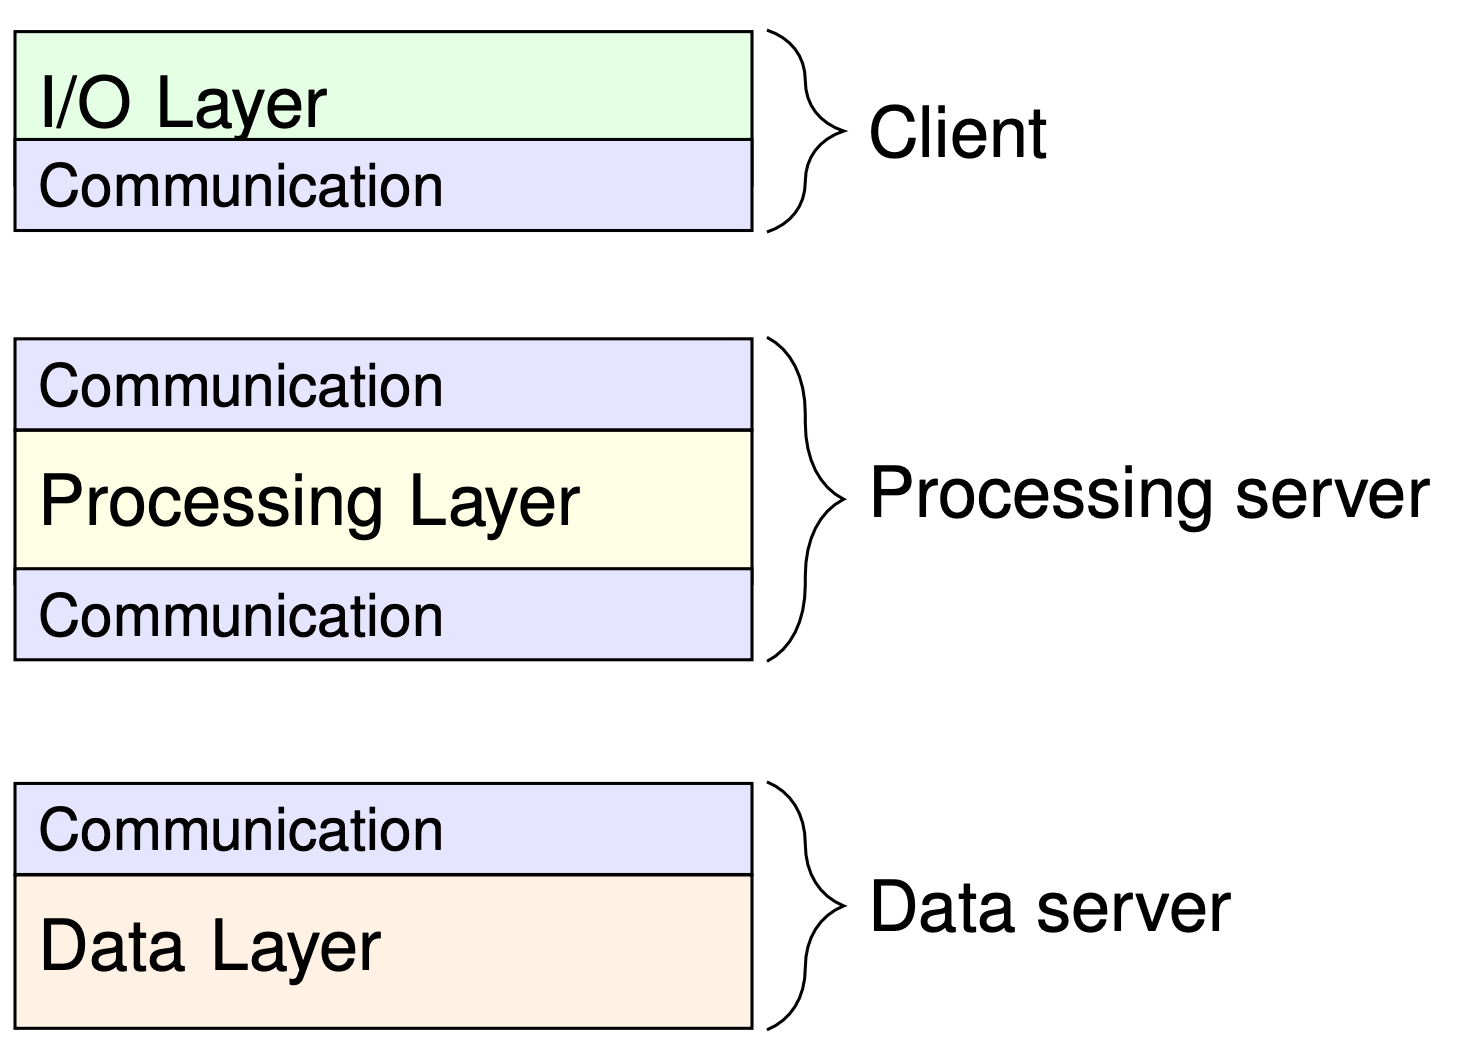
\includegraphics[scale=0.125]{three-tear-client-server.png}	
\end{table}

$\bold{Broker}$
\begin{table}[H]
\caption{Broker}
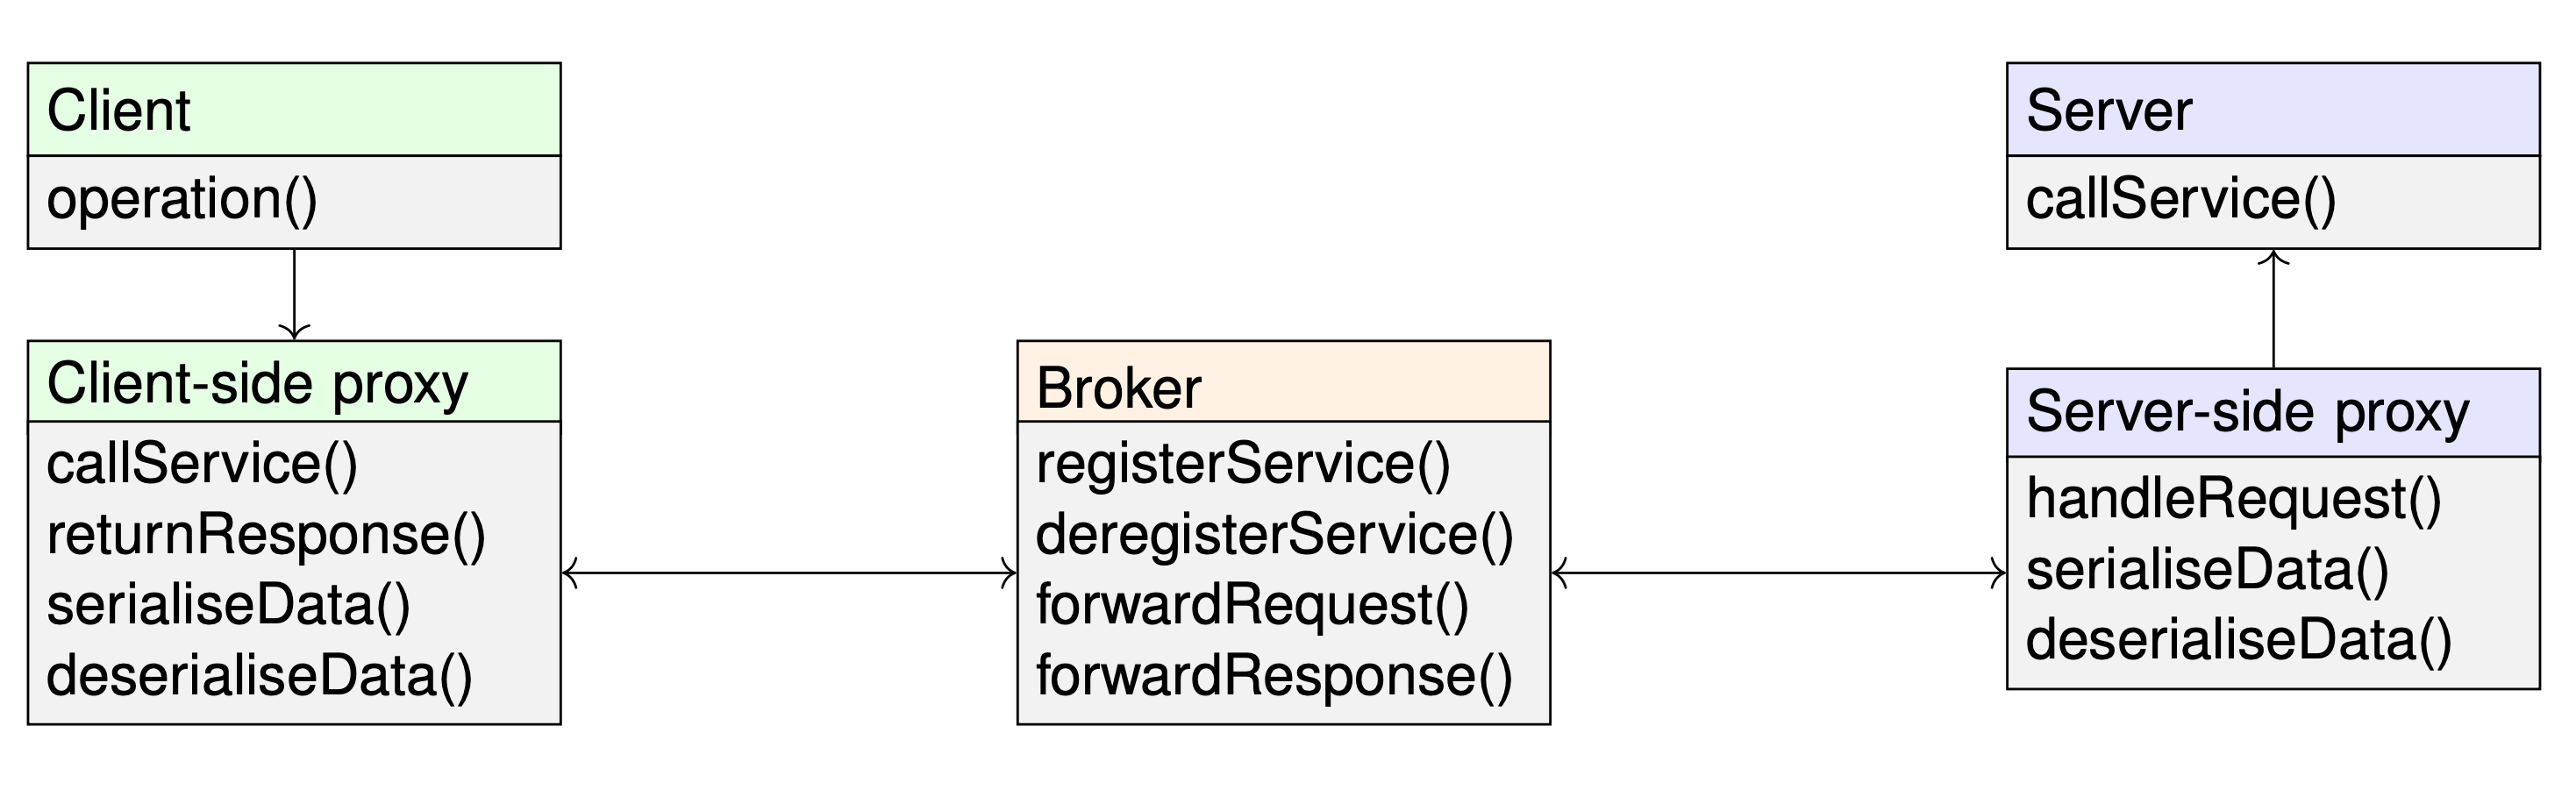
\includegraphics[scale=0.125]{Broker.png}	
\end{table}
\begin{multicols}{2}
$\bold{Pros}$:
\begin{itemize}
	\item Separation of concerns
	\item Stabilität
	\item Räumliche Unabhängigkeit 
	\item Plattform-Unabhängigkeit
\end{itemize}
\columnbreak
$\bold{Cons}$:
\begin{itemize}
	\item Fehlertoleranz ist nötig
	\item Indirekte Kommunikation führt zu Performanceverlust
	\item Potenzieller Flaschenhals beim Broker
	\item Proxies sind von Broker abhänig
\end{itemize}
\end{multicols}
$\bold{Verwendung}$
\begin{itemize}
	\item Client und Server müssen entkoppelt sein
	\item Komponenten müssen Services durch Servicenamen erreichen
	\item Komponenten ändern sich während der Laufzeit
	\item Implementationsdetaills von Client und Server müssen verborgen bleiben
\end{itemize}






